\chapter{Giới thiệu}
\label{ch:gioi-thieu}

\section{Bối cảnh và vấn đề nghiên cứu}
\label{sec:boi-canh}

Rối loạn trầm cảm (Major Depressive Disorder -- MDD) là một trong những nguyên nhân phổ biến gây suy giảm chất lượng cuộc sống và gia tăng gánh nặng y tế cộng đồng trên quy mô toàn cầu \cite{pratt2014depression}. Theo Tổ chức Y tế Thế giới (WHO), hàng trăm triệu người thuộc nhiều lứa tuổi đang phải đối mặt với các mức độ triệu chứng trầm cảm khác nhau. Không chỉ ảnh hưởng tiêu cực đến sức khỏe tinh thần, năng suất học tập, làm việc và gắn kết gia đình, trầm cảm mức độ nặng còn liên quan mật thiết đến nguy cơ tự tử. Đáng chú ý, nhiều người có triệu chứng ở giai đoạn đầu hoặc mức độ nhẹ thường không nhận biết được tình trạng của mình, hoặc e ngại rào cản tâm lý xã hội (stigma), dẫn đến việc chậm trễ tiếp cận các dịch vụ hỗ trợ y tế.

Trong thực hành lâm sàng và các nghiên cứu dịch tễ học, công cụ phổ biến nhất để sàng lọc và đánh giá mức độ triệu chứng trầm cảm là Thang đo Sức khỏe Bệnh nhân 9 mục (Patient Health Questionnaire-9 -- PHQ-9) do Kroenke và cộng sự phát triển \cite{kroenke2001phq, spitzer1999validation}. PHQ-9 gồm 9 câu hỏi tự điền tương ứng với các tiêu chuẩn triệu chứng trong Sổ tay Chẩn đoán và Thống kê Rối loạn Tâm thần (DSM-IV). Mỗi câu hỏi được tính từ 0 đến 3 điểm, tạo nên tổng điểm dao động từ 0 đến 27 điểm. Trong y văn, thang điểm này thường được chia thành năm khoảng mức độ: Tối thiểu (Minimal, 0--4 điểm), Nhẹ (Mild, 5--9 điểm), Vừa (Moderate, 10--14 điểm), Nặng vừa (Moderately severe, 15--19 điểm) và Nặng (Severe, 20--27 điểm).

Mặc dù PHQ-9 có độ tin cậy sàng lọc cao, phương pháp này vẫn phụ thuộc vào bản chất tự báo cáo (self-reported questionnaire). Người tham gia khảo sát có thể khai báo chưa đầy đủ hoặc không nhất quán do tâm lý chủ quan hay định kiến cá nhân. Vì vậy, việc tìm hiểu khả năng khai thác các chỉ số khách quan từ hồ sơ kiểm tra sức khỏe thể chất và xét nghiệm cận lâm sàng dạng bảng để hỗ trợ sàng lọc mức độ triệu chứng là một hướng nghiên cứu đáng quan tâm trong y tế dự phòng và chăm sóc sức khỏe ban đầu.

Các cuộc điều tra sức khỏe quy mô dân số, tiêu biểu là Khảo sát Sức khỏe và Dinh dưỡng Quốc gia Hoa Kỳ (National Health and Nutrition Examination Survey -- NHANES) do CDC thực hiện định kỳ hai năm một lần \cite{cdc2014nhanes, cdc2016nhanes}, cung cấp nguồn dữ liệu dạng bảng phong phú. NHANES kết hợp phỏng vấn nhân khẩu, thăm khám thể lực và các xét nghiệm sinh hóa máu chuẩn hóa. Một số nghiên cứu y sinh học đã ghi nhận mối liên hệ gián tiếp giữa triệu chứng trầm cảm và các chỉ số chuyển hóa toàn thân, bao gồm phản ứng viêm thể nhẹ, nồng độ lipid máu, huyết áp và chỉ số khối cơ thể (BMI).

Học máy (Machine Learning -- ML) là công cụ phù hợp để tìm kiếm các mối quan hệ phi tuyến giữa các chỉ số sinh lý đa biến. Tuy nhiên, khi áp dụng Machine Learning vào bài toán dự đoán mức độ triệu chứng PHQ-9 trên dữ liệu khảo sát cộng đồng dạng bảng, các mô hình phải đối mặt với ba thách thức kỹ thuật lớn:
\begin{enumerate}
    \item \textbf{Mất cân bằng lớp (Severe Class Imbalance):} Trong quần thể dân cư nói chung, phần lớn người tham gia khảo sát thuộc nhóm triệu chứng tối thiểu ($C_0$, chiếm khoảng 74--76\%), trong khi nhóm có triệu chứng nặng ($C_4$) chỉ chiếm khoảng 1.0--1.3\%. Sự chênh lệch này khiến các mô hình học máy thông thường có xu hướng dự đoán nghiêng về lớp đa số để đạt độ chính xác tổng thể (Accuracy) cao nhưng bỏ sót các ca có triệu chứng thực tế.
    \item \textbf{Chồng lấn phân phối đặc trưng (High Feature Overlap):} Khác với các bệnh lý có chỉ dấu sinh học đặc hiệu trong máu, các chỉ số sinh lý ngoại vi giữa người có triệu chứng tối thiểu và người có triệu chứng nhẹ phân tán rộng và chồng lấn đáng kể. Ranh giới phân tách trong không gian đặc trưng trở nên mờ nhạt, khiến các mô hình phân loại phẳng dễ nhầm lẫn giữa các mức độ kế cận.
    \item \textbf{Suy giảm hiệu năng theo độ chi tiết nhãn (Granularity Degradation):} Phần lớn các công trình trước đây tập trung vào bài toán phân loại nhị phân ($T_2$: Không có triệu chứng vs Có triệu chứng). Khi mở rộng bài toán sang phân loại đa mức ($T_3, T_4, T_5$) để phục vụ phân tầng chi tiết hơn, hiệu năng của các thuật toán học máy giảm rõ rệt.
\end{enumerate}

Xuất phát từ các vấn đề thực tế trên, đề tài \textbf{“Nghiên cứu khung học máy cho dự đoán mức độ triệu chứng trầm cảm từ dữ liệu sinh lý”} được thực hiện nhằm xây dựng và đánh giá khung thực nghiệm \textbf{DepSev-ML} (Depression Severity Machine Learning). Cần lưu ý rằng, nghiên cứu này không hướng tới việc thay thế bảng câu hỏi PHQ-9 hay đưa ra chẩn đoán lâm sàng tự động thay bác sĩ tâm thần, mà tập trung làm rõ giới hạn dự đoán của các đặc trưng sinh lý dạng bảng và thử nghiệm các kiến trúc học máy phù hợp nhằm cải thiện độ nhạy cho các nhóm có triệu chứng.

\section{Phát biểu bài toán}
\label{sec:phat-bieu-bai-toan}

Bài toán nghiên cứu của DepSev-ML được xây dựng dưới dạng bài toán học có giám sát (Supervised Learning) trên dữ liệu dạng bảng.

Cho tập dữ liệu gồm $N$ mẫu quan sát độc lập:
\begin{equation}
    \mathcal{D} = \{(\mathbf{x}_i, s_i)\}_{i=1}^N
\end{equation}
trong đó:
\begin{itemize}
    \item $\mathbf{x}_i \in \mathcal{X} \subseteq \mathbb{R}^d$ là vectơ đặc trưng $d$ chiều của đối tượng thứ $i$, bao gồm các biến số đo lường thể chất (nhân trắc học, huyết áp), xét nghiệm sinh hóa máu, thông tin lối sống (hoạt động thể lực, giấc ngủ, hút thuốc, rượu bia) và nhân khẩu học.
    \item $s_i \in \{0, 1, \dots, 27\}$ là tổng điểm PHQ-9 của đối tượng thứ $i$, được tính bằng tổng của 9 câu hỏi thành phần:
    \begin{equation}
        s_i = \sum_{j=1}^9 \text{DPQ}_{ij}, \quad \text{với } \text{DPQ}_{ij} \in \{0, 1, 2, 3\}
    \end{equation}
\end{itemize}

Nhãn mục tiêu $y_i$ được xác định thông qua ánh xạ lượng giá $\Phi: \{0, \dots, 27\} \to \mathcal{Y}_K$, với $\mathcal{Y}_K = \{0, 1, \dots, K-1\}$ là không gian đầu ra gồm $K$ mức độ rời rạc ($K \in \{2, 3, 4, 5\}$):
\begin{itemize}
    \item \textbf{Thiết lập $T_2$ ($K=2$, Phân loại nhị phân):} $y_i = 0$ nếu $s_i \in [0, 4]$ (Tối thiểu); $y_i = 1$ nếu $s_i \in [5, 27]$ (Có triệu chứng).
    \item \textbf{Thiết lập $T_3$ ($K=3$, Ba nhóm theo quy ước nghiên cứu):} $y_i = 0$ nếu $s_i \in [0, 4]$ ($C_0$: Tối thiểu); $y_i = 1$ nếu $s_i \in [5, 9]$ ($C_1$: Nhẹ); $y_i = 2$ nếu $s_i \in [10, 27]$ ($C_2^+$: Nặng theo quy ước).
    \item \textbf{Thiết lập $T_4$ ($K=4$, Bốn mức độ):} $C_0$ ($0$--$4$), $C_1$ ($5$--$9$), $C_2$ ($10$--$14$), $C_3^+$ ($15$--$27$).
    \item \textbf{Thiết lập $T_5$ ($K=5$, Năm mức độ chuẩn PHQ-9):} $C_0$ (Minimal, $0$--$4$), $C_1$ (Mild, $5$--$9$), $C_2$ (Moderate, $10$--$14$), $C_3$ (Moderately severe, $15$--$19$), và $C_4$ (Severe, $20$--$27$).
\end{itemize}

Mục tiêu là huấn luyện hàm dự đoán $f: \mathcal{X} \to \mathcal{Y}_K$ nhằm tối ưu hóa khả năng nhận diện trên tất cả các lớp. Do dữ liệu mất cân bằng lớp rõ rệt, nghiên cứu ưu tiên hai chỉ số đánh giá chính:
\begin{equation}
    \text{Macro-F1} = \frac{1}{K} \sum_{k=0}^{K-1} \text{F1}_k = \frac{1}{K} \sum_{k=0}^{K-1} \frac{2 \cdot \text{Precision}_k \cdot \text{Recall}_k}{\text{Precision}_k + \text{Recall}_k}
\end{equation}
\begin{equation}
    \text{Balanced Accuracy} = \frac{1}{K} \sum_{k=0}^{K-1} \text{Recall}_k
\end{equation}

Sơ đồ tổng quan về bài toán và luồng xử lý của nghiên cứu được thể hiện trong Hình \ref{fig:problem-formulation}.

\begin{figure}[htbp]{Sơ đồ tổng quan phát biểu bài toán và luồng xử lý của khung học máy DepSev-ML}
\centering
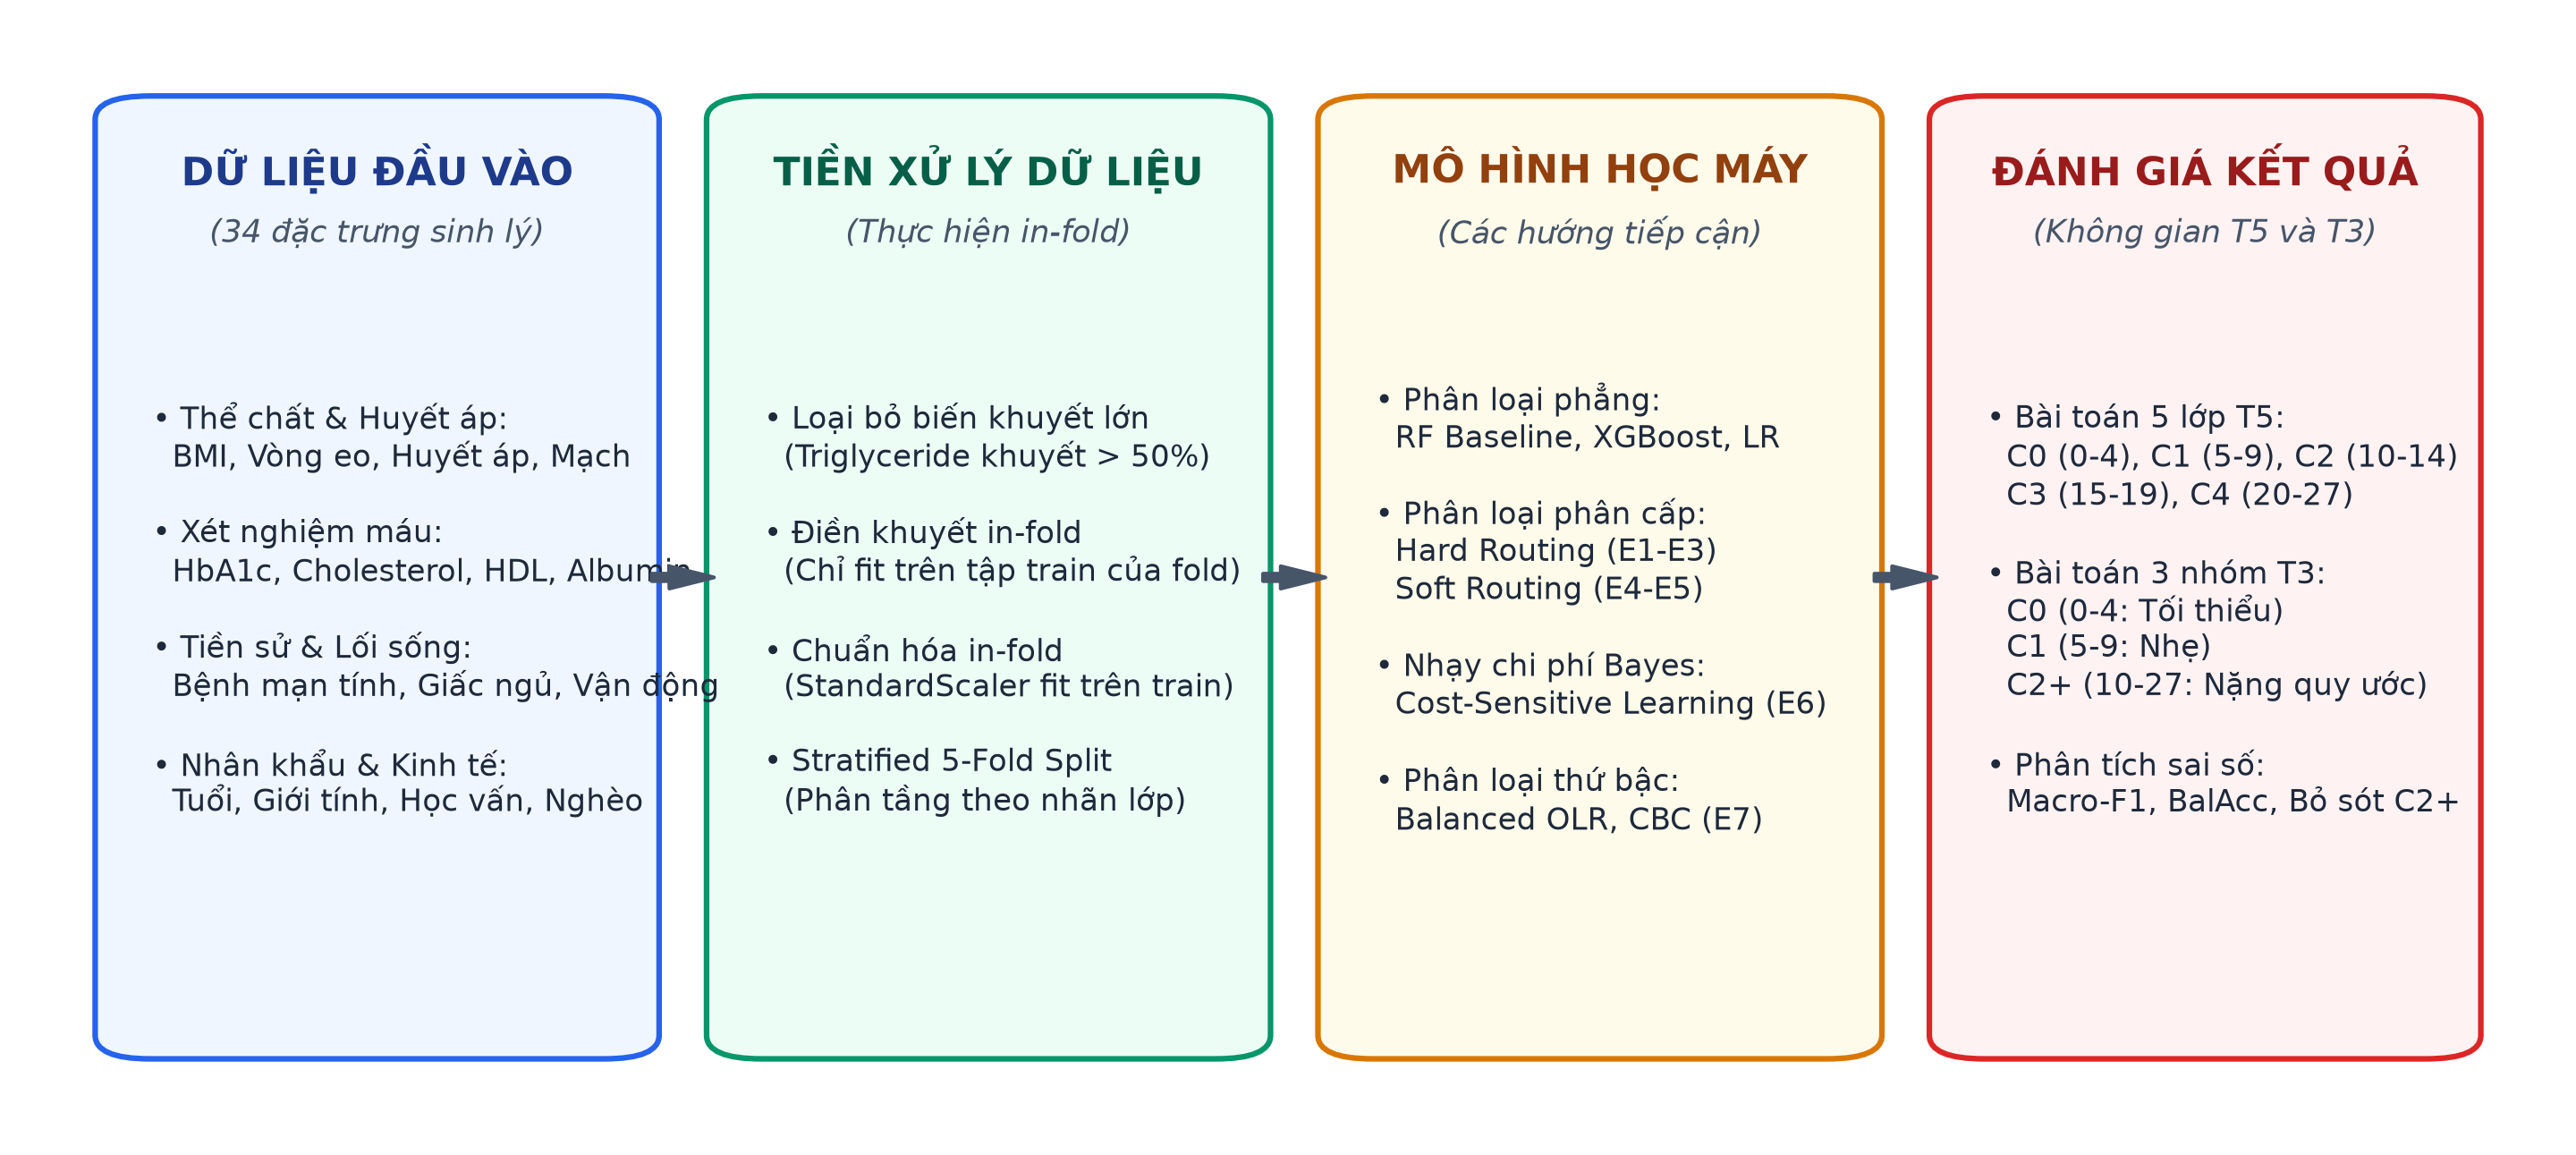
\includegraphics[width=\textwidth]{figures/fig1_problem_formulation.png}
\label{fig:problem-formulation}
\end{figure}
\FloatBarrier

\textbf{Nguyên tắc kiểm soát rò rỉ dữ liệu in-fold (In-Fold Preprocessing):} Để kết quả đánh giá phản ánh đúng khả năng khái quát hóa trên dữ liệu chưa thấy, ma trận đặc trưng đầu vào $\mathbf{X}$ không chứa bất kỳ câu hỏi nào trong 9 mục khảo sát DPQ. Tất cả các bước chuẩn hóa, điền khuyết (imputation) và mã hóa đặc trưng đều được học độc lập trên tập huấn luyện của từng fold kiểm định chéo và áp dụng nhất quán sang tập kiểm tra tương ứng.

\section{Mục tiêu và câu hỏi nghiên cứu}
\label{sec:muc-tieu-va-cau-hoi}

Mục tiêu tổng quát của đề tài là xây dựng một quy trình thực nghiệm học máy rõ ràng, có khả năng tái lập, nhằm khảo sát hiệu năng và giới hạn của việc dự đoán mức độ triệu chứng trầm cảm từ dữ liệu sinh lý NHANES.

Đề tài tập trung trả lời năm câu hỏi nghiên cứu (Research Questions -- RQ):
\begin{itemize}
    \item \textbf{RQ1 (Đóng góp của các nhóm đặc trưng):} Những nhóm đặc trưng nào (trong số nhân trắc, huyết áp, xét nghiệm máu, lối sống và nhân khẩu học) đóng góp nhiều nhất vào khả năng phân loại mức độ PHQ-9, và việc kết hợp các nhóm này có cải thiện hiệu năng so với từng nhóm riêng rẽ không?
    \item \textbf{RQ2 (Xu hướng suy giảm theo độ chi tiết nhãn):} Hiệu năng mô hình thay đổi ra sao khi tăng số lớp từ 2 lên 3, 4 và 5 mức độ? Ranh giới phân lớp nào gây ra mức sụt giảm lớn nhất?
    \item \textbf{RQ3 (Ảnh hưởng của việc tăng quy mô dữ liệu):} Việc mở rộng cỡ mẫu từ một chu kỳ đơn lẻ ($N = 5.054$) lên ba chu kỳ gộp ($N = 14.581$) với các đặc trưng hài hòa có giúp cải thiện hiệu năng ở các mức độ chi tiết hay không?
    \item \textbf{RQ4 (Hiệu quả của phân loại phân cấp hai bước):} Kiến trúc phân loại phân cấp (Hierarchical Classification) trên không gian 3 nhóm ($T_3$) thể hiện ra sao so với phân loại phẳng truyền thống (Flat Classification), và cơ chế định tuyến cứng (Hard Routing) dẫn đến sai số một chiều như thế nào?
    \item \textbf{RQ5 (Vai trò của Soft, Cost-Sensitive và Ordinal Classification):} Việc áp dụng định tuyến mềm (Soft Voting Fusion), lý thuyết quyết định nhạy chi phí Bayes và phân loại thứ bậc (Ordinal Classification) giúp điều chỉnh sự đánh đổi giữa Macro-F1, Balanced Accuracy và số ca nặng bị bỏ sót như thế nào?
\end{itemize}

\section{Phạm vi và giới hạn nghiên cứu}
\label{sec:pham-vi-nghien-cuu}

Các giới hạn nghiên cứu của đề tài bao gồm:
\begin{enumerate}
    \item \textbf{Nguồn dữ liệu:} Nghiên cứu sử dụng dữ liệu khảo sát cắt ngang dạng bảng của NHANES (Hoa Kỳ) các chu kỳ 2011--2012, 2013--2014 và 2015--2016, áp dụng cho người tham gia từ 20 tuổi trở lên có đủ 9 mục khảo sát PHQ-9.
    \item \textbf{Dạng đặc trưng:} Đề tài chỉ sử dụng các đặc trưng sinh lý, cận lâm sàng và nhân khẩu dạng bảng trích xuất từ hồ sơ khám sức khỏe định kỳ. Nghiên cứu \textbf{không sử dụng tín hiệu chuỗi thời gian thô} như điện tâm đồ (ECG) hay điện não đồ (EEG).
    \item \textbf{Mục đích sử dụng:} Đề tài tập trung vào bài toán sàng lọc mức độ triệu chứng tự báo cáo trong nghiên cứu dịch tễ học, \textbf{không phải công cụ chẩn đoán bệnh học lâm sàng}. Kết quả dự đoán không thay thế quy trình thăm khám và đánh giá của bác sĩ tâm thần.
    \item \textbf{Phương pháp học máy:} Nghiên cứu tập trung thử nghiệm và so sánh các kiến trúc mô hình học máy dạng bảng (phẳng, phân cấp, nhạy chi phí và thứ bậc) để tìm hiểu đặc điểm dữ liệu thực tế.
\end{enumerate}

\section{Phương pháp tiếp cận và tiến trình nghiên cứu hai giai đoạn}
\label{sec:dong-gop-nghien-cuu}

Nghiên cứu được triển khai qua hai giai đoạn kế tiếp nhau, được minh họa trong Hình \ref{fig:research-progression}.

\begin{figure}[htbp]{Sơ đồ quy trình nghiên cứu: Từ khảo sát 5 mức độ $T_5$ đến mô hình phân cấp $T_3$}
\centering
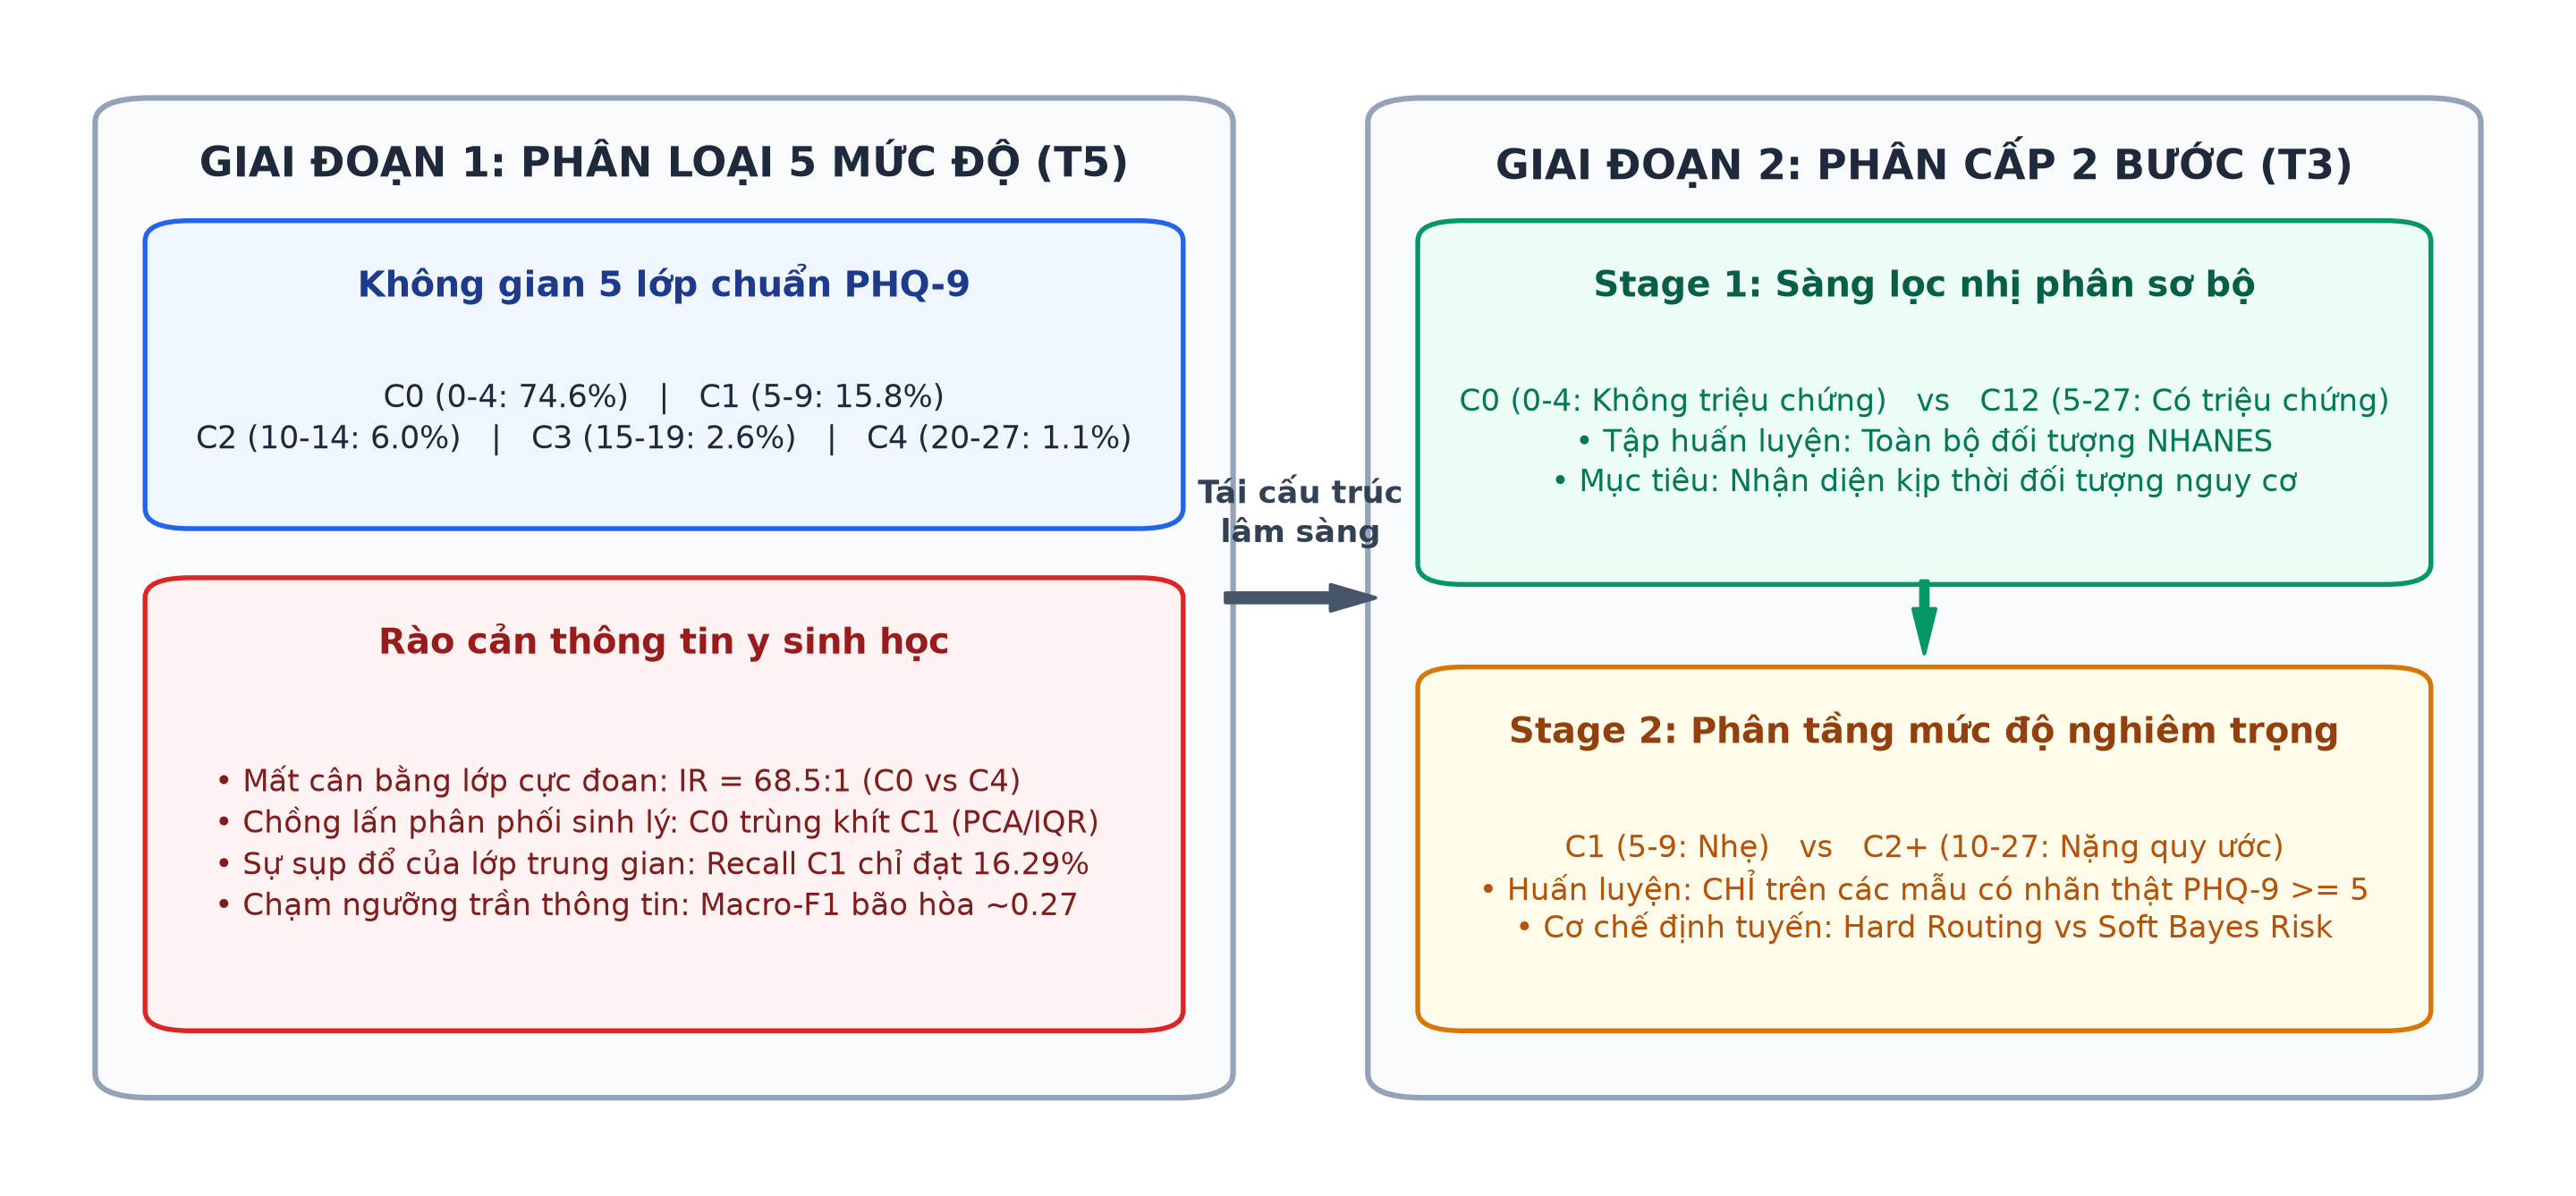
\includegraphics[width=\textwidth]{figures/fig_research_progression_t5_to_t3.png}
\label{fig:research-progression}
\end{figure}
\FloatBarrier

\begin{enumerate}
    \item \textbf{Giai đoạn 1 -- Khảo sát trên không gian 5 mức độ chuẩn PHQ-9 ($T_5$):} 
    Nghiên cứu bắt đầu bằng việc xây dựng mô hình cơ sở với 4 thuật toán học máy phổ biến gồm Logistic Regression, Decision Tree, Random Forest và XGBoost để dự đoán năm mức độ triệu chứng ($C_0$: $0$--$4$, $C_1$: $5$--$9$, $C_2$: $10$--$14$, $C_3$: $15$--$19$, $C_4$: $20$--$27$). Kết quả giai đoạn này cho thấy: (1) Dữ liệu mất cân bằng lớn giữa lớp $C_0$ (74.6\%) và lớp $C_4$ (1.1\%); (2) Khả năng nhận diện của mô hình trên các lớp thiểu số rất thấp, đặc biệt lớp $C_1$ có Recall chỉ đạt 15.83\% (hơn 53.9\% bị nhầm thành $C_0$) và lớp $C_4$ chỉ nhận diện đúng 1/44 ca (Recall = 2.27\%); (3) Sự chồng lấn phân phối của các chỉ số sinh lý khiến hiệu năng của các mô hình trên $T_5$ dao động quanh mức Macro-F1 $\approx 0.27$, ngay cả khi tăng cỡ mẫu lên 14.581 quan sát.
    \item \textbf{Giai đoạn 2 -- Thử nghiệm phân loại phân cấp hai bước trên không gian 3 nhóm ($T_3$):} 
    Từ những hạn chế quan sát được ở bài toán 5 lớp, nghiên cứu chuyển hướng sang bài toán phân loại 3 nhóm ($C_0$: Tối thiểu, $C_1$: Nhẹ, $C_2^+$: Nặng theo quy ước nghiên cứu, với điểm PHQ-9 $\ge 10$) thông qua kiến trúc hai bước:
    \begin{itemize}
        \item \textit{Stage 1 (Sàng lọc sơ bộ):} Phân loại nhị phân để nhận diện đối tượng có triệu chứng ($C_0$ vs $C_{12} = C_1 \cup C_2^+$), huấn luyện trên tập dữ liệu đầy đủ.
        \item \textit{Stage 2 (Phân tầng mức độ):} Phân loại giữa mức Nhẹ ($C_1$) và Nặng theo quy ước ($C_2^+$). Về mặt phương pháp, Stage 2 được huấn luyện \textbf{chỉ trên các mẫu có nhãn thật $\text{PHQ-9} \ge 5$}. Khi suy luận, các mẫu được chuyển sang Stage 2 thông qua định tuyến cứng (Hard Routing) hoặc định tuyến mềm kết hợp chi phí rủi ro Bayes (Soft Bayes Risk).
    \end{itemize}
    Cần nêu rõ rằng $T_3$ là một bài toán phân loại khác với $T_5$, không phải là kết quả cải thiện trực tiếp trên cùng không gian 5 lớp.
\end{enumerate}

Những đóng góp chính của đề tài bao gồm:
\begin{enumerate}
    \item \textbf{Đánh giá thực nghiệm có kiểm soát về đóng góp của các nhóm đặc trưng:} Xây dựng quy trình đánh giá 4 thuật toán trên các không gian đặc trưng lũy tiến ($F_1 \to F_4$), làm rõ vai trò bổ trợ của tiền sử bệnh lý mạn tính, hành vi lối sống và nhân khẩu học so với các chỉ số cận lâm sàng ngoại vi đơn thuần.
    \item \textbf{Khảo sát và lượng hóa sự suy giảm hiệu năng theo độ chi tiết nhãn:} Khảo sát sự biến thiên hiệu năng từ bài toán nhị phân $T_2$ sang các bài toán đa mức $T_3, T_4, T_5$, kết hợp phân tích tương quan và trực quan hóa PCA để giải thích nguyên nhân gây suy giảm nhận diện tại các ranh giới lớp liền kề.
    \item \textbf{Phân tích điểm nghẽn sai số và thử nghiệm mô hình nhạy chi phí:} Phân tích cơ chế lan truyền sai số một chiều trong cấu trúc phân cấp định tuyến cứng ($T_3$); qua đó đề xuất mô hình phân cấp mềm kết hợp lý thuyết quyết định nhạy chi phí Bayes nhằm hạn chế bỏ sót các ca có triệu chứng nặng.
    \item \textbf{Đánh giá hướng tiếp cận thứ bậc và kiểm định ngoại suy theo thời gian:} Khảo sát các mô hình Ordinal Classification nhằm khai thác mối quan hệ thứ bậc tự nhiên của thang đo PHQ-9, đồng thời kiểm tra độ ổn định của mô hình qua giao thức kiểm định ngoại suy trên chu kỳ khảo sát độc lập.
\end{enumerate}

\section{Cấu trúc báo cáo}
\label{sec:bo-cuc-khoa-luan}

Báo cáo dự án nghiên cứu gồm 5 chương:
\begin{itemize}
    \item \textbf{Chương 1: Giới thiệu} -- Trình bày bối cảnh nghiên cứu, phát biểu bài toán, mục tiêu, 5 câu hỏi nghiên cứu, phạm vi và tiến trình thực hiện.
    \item \textbf{Chương 2: Cơ sở lý thuyết và các nghiên cứu liên quan} -- Giới thiệu thang đo PHQ-9, đặc tính mất cân bằng lớp và chồng lấn đặc trưng trong dữ liệu y tế dạng bảng, thuật toán Random Forest và các hướng mô hình hóa (phẳng, phân cấp, thứ bậc).
    \item \textbf{Chương 3: Dữ liệu và phương pháp nghiên cứu} -- Trình bày nguồn dữ liệu NHANES, quy trình tiền xử lý, hệ thống 4 nhóm đặc trưng, các cấu hình mô hình thực nghiệm ($E_0 \to E_7$) và quy trình kiểm định chéo.
    \item \textbf{Chương 4: Thực nghiệm và thảo luận} -- Trình bày chi tiết các kết quả Feature Ablation, tối ưu hóa siêu tham số, phân tích độ chi tiết nhãn, mở rộng đa chu kỳ, so sánh các mô hình $E_0 \to E_7$ và kiểm định theo thời gian.
    \item \textbf{Chương 5: Kết luận và hướng phát triển} -- Tóm tắt các kết quả đạt được, thảo luận các giới hạn của dữ liệu và đề xuất hướng nghiên cứu tiếp theo.
\end{itemize}
